\chapter{Green's Functions at Zero Temperature}
The Green's function is a method trying to deduce the properties of some system described by a Hamiltonian $H$ which may not solved exactly. The usual approach is to set
%
\begin{equation}\label{2.1}
H= H_0 + V
\end{equation}
%
where $H_0$ is the Hamiltonian can be solved exactly.
The term $V$ represents all remaining parts of $H$.
One tries to choose $H_0$ so that the effects $V$ are small.
The basic procedure is to start with a system completely described by $H_0$.
The effects of V are introduced, and then calculations are done to find how $V$ changes the properties.
These steps are the basic procedure in many-body theory.

\section{Interaction representation}\label{s2.1}
\subsection{Schr\"{o}dinger}
In Schr\"{o}dinger representation
%
\begin{equation}\label{2.2}
i\partial_t\psi(t) = H\psi(t)
\end{equation}
with the formal operator solution
\begin{equation}\label{2.3}
\psi(t) = e^{-i H t}\psi(0)
\end{equation}

The use of this formula requires:
\begin{itemize}
  \item The wavefunction is time dependent.
  \item Operators such as the Hamiltonian $H$ are taken to be independent of time.
\end{itemize}

\subsection{Heisenberg}
The Heisenberg representation has the following properties:
\begin{itemize}
  \item The wavefunction is independent of the time
  \item The operators are time dependent and given by
  \begin{equation}\label{2.4}
    O(t)=e^{i H t}O(0) e^{-i Ht}
  \end{equation}
  or, equivalently, the equation of motion is given by
  \begin{equation}
    \label{2.5}
    i\partial_t O(t) = [O(t),H]
  \end{equation}
\end{itemize}

In physics, one is usually trying to evaluate matrix elements in order to determine the transition rates, in different representation
\begin{equation}
  \label{2.6}
  \langle \psi^\dagger_1(t) O \psi_2(t)\rangle_S = \langle \psi^\dagger_1 O(t) \psi_2 \rangle_H = \langle \psi^\dagger_1(0) e^{i Ht} O(0) e^{-i Ht} \psi_2(0) \rangle
\end{equation}

\subsection{Interaction}
The interaction representation is another way of doing things.
{\bf Here both the wavefunction and operators are time dependent.}
The Hamiltonian is given by
\begin{equation}
H= H_0 +V \label{2.8}
\end{equation}
In the whole book the wavefunction and operator in interaction picture will represents by a caret.
They have the following properties:
\begin{itemize}
\item The operators have a time dependence:
\begin{equation}
  \hat{O}(t) = e^{iH_0 t}O_S e^{-iH_0 t} ~ ~ ~ ~ i\partial_t \hat{O}(t) = [\hat{O}(t),H_0]\label{2.9}
\end{equation}
\item The wavefunction have the time dependence:
\begin{equation}
  \hat{\psi}(t) = e^{iH_0 t}e^{-iHt} \psi(0) \label{2.10}
\end{equation}
It is assumed that $[H_0,V]\neq 0$, which result a non-trivial problem.
\end{itemize}
Similarly, the matrix elements give the same result.
The time dependence of the operator is relaying on the unperturbed Hamiltonian as in \eqref{2.9}.
For the dependence of the wavefunction is governed by
\begin{equation}
  \partial_t \hat{\psi}(t) = -i\hat{V}(t) \hat{\psi}(t) \label{2.13}
\end{equation}
As operator was introduced into \eqref{2.10}, which can be defined as
\begin{equation}
  U(t) = e^{iH_0 t} e^{-i Ht} \label{2.14}
\end{equation}
Furthermore, it obeys a differential equation which can be written in the interaction representation:
\begin{equation}
  \partial_t U(t) = -i \hat{V}(t) U(t) \label{2.15}
\end{equation}
By setting the initial condition $U(0)=1$, we can have this iterated relation
\begin{eqnarray}\label{2.18}
  U(t)&=&1-i\int_0^t dt_1 \hat{V}(t_1)U(t_1)\\
  &=& \sum_{n=0}^\infty (-i)^n \int_0^t dt_1 \int_0^{t_1} dt_2 \dots \int_0^{t_{n-1}} dt_n \hat{V}(t_1) \hat{V}(t_2) \dots \hat{V}(t_n) \nonumber
\end{eqnarray}
In this situation, it is convenient to introduce the time-ordering operator $T$, which works on a group of time-dependent operators.
With the help of time-ordering operator, the expansion of $U(t)$ gives
\begin{equation}
  U(t)=1 + \sum_{n=1}^\infty \frac{(-i)^n}{n!} \int_0^t dt_1 \dots \int_0^{t_{n-1}} dt_n T[ \hat{V}(t_1)\dots \hat{V}(t_n) ] \label{2.26}
\end{equation}
This expansion may be abbreviated by writing it as
\begin{equation}\label{2.27}
  U(t) = T \exp \left[ -i \int_0^t dt_1 \hat{V}(t_1) \right]
\end{equation}
Always keep in minds that this is a short hand for the series definition.

\section{S Matrix}\label{s2.2}
It had been shown that the wavefunction in interaction representation had a time dependence at zero time:
\begin{equation}
  \hat{\psi}(t) = U(t_) \hat{\psi}(0) \label{2.28}
\end{equation}
Now define the $S$ matrix as the operator $S(t,t')$ which changes the wavefunction in two different time
\begin{equation}
  \hat{\psi}(t) = S(t,t') \hat{\psi}(t') \label{2.29}
\end{equation}
with the definition
\begin{equation}
  S(t,t')=U(t)U^\dagger(t') \label{2.31}
\end{equation}
and some important properties of this operators
\begin{itemize}
  \item $S(t,t)=1$
  \item $S^\dagger(t,t') = S(t',t)$
  \item $S(t,t')S(t',t")=S(t,t")$
\end{itemize}
Finally, it can also be expressed as a time-ordered operator by
\begin{equation}
  S(t,t') =T \exp [ -i \int_{t'}^t dt_1 \hat{V}(t_1) ] \label{2.33}
\end{equation}

In different representation, the wavefunction is identical at the $t=0$, let $\psi(0)$ as the exact ground state wavefunction, and $\phi_0$ as the ground state of $H_0$.
The relationship between these tow ground states at zero temperature was established by Gell-Mann and Low
\begin{equation}
  \psi(0) = S(0,-\infty)\phi_0 \label{2.36}
\end{equation}
The result can be regard as the following, since
\begin{equation}
  \hat{\psi}(t) = S(t,0) \psi(0)
\end{equation}
operate by $S(0,t)$ we can get
\begin{equation}
  \psi(0) = S(0,t) \hat{\psi}(t)
\end{equation}
Let $t \to -\infty$, one get
\begin{equation}
  \psi(0) = S(0,-\infty) \hat{\psi}(-\infty) \label{2.39}
\end{equation}
The important assertion is that $\hat{\psi}(-\infty)=\phi_0$.
The traditional argument is that one stats in the long past with the wavefunction $\phi_0$ which does not contain the effects of interaction $V$.
The operator $S$ brings this wavefunction \textit{adiabatically} up to the present which with the interaction.

Additional property of these states which is needed for the discussion of Green's function is , as $t\to +\infty$,
\begin{equation}
  \hat{\psi}(\infty) = S(\infty,0) \psi(0)  \label{2.40}
\end{equation}
One possible assumption is that $\hat{\psi}(\infty)$ must be related to $\phi_0$.
If they are equal except for a phase factor $L$
\begin{eqnarray}
  &&\phi_0 e^{iL} = \hat{\psi}(\infty) = S(\infty,0)\psi(0) = S(\infty,-\infty)\phi_0
  \label{2.41}\\
  &&e^{iL} = \bra{\phi_0} S(\infty,-\infty) \ket{\phi_0} \label{2.42}
\end{eqnarray}

\section{Green's Function}\label{s2.3}
At zero temperature the electron Green's function is defined as
\begin{equation}
  G(\lambda,t-t') = -i \bra{}TC_\lambda(t) C_\lambda^\dagger(t') \ket{} \label{2.43}
\end{equation}
The quantum number $\lambda$ can be anything depending on the problem\footnote{For free-electron gas $\lambda = (\mathbf{p},\sigma)$, where is wave vector and spin.}.
At zero temperature the state $\ket{}$ must be the ground state.

In the definition of Green's function the $C_\lambda$ represent states of $H_0$, while the ground state $\ket{}$ is an eigenstate of $H$.
Furthermore, \eqref{2.43} is defined in Heisenberg picture, one have the usual dependence of time on operators \eqref{2.4}.

To change the Green's function from Heisenberg picture to interaction one.
Let $\ket{\phi_0}$ be the ground state of $H_0$, so we have
\begin{equation}
  \ket{} = S(0,-\infty) \ket{\phi_0} \label{2.48}
\end{equation}
Next change the operators to interaction representation\footnote{
From the \eqref{2.4} and $\eqref{2.8}$ we get:
\begin{eqnarray*}
  &&C_\lambda(t) = e^{iHt}e^{-iH_0 t}\hat{C}_\lambda(t)e^{iH_0 t}e^{-iHt} \\
  &&= U^\dagger(t)\hat{C}_\lambda(t)U(t) = S(0,t)\hat{C}_\lambda(t)S(t,0)
\end{eqnarray*}
}
, we have the Green's function
\begin{eqnarray*}
G(\lambda,t-t') &=& -i\Theta(t-t')\bra{\phi_0} S(-\infty,0)S(0,t)\hat{C}_\lambda(t)S(t,0) S(0,t')\\
&&\times\hat{C}_\lambda^\dagger(t') S(t',0)S(0,-\infty)\ket{\phi_0} \\
&&+ i\Theta(t-t') \bra{\phi_0} S(-\infty,0) S(0,t')\hat{C}_\lambda^\dagger(t')S(t',0) S(0,t)\\
&&\times\hat{C}_\lambda(t)S(t,0)S(0,-\infty)\ket{\phi_0}
\end{eqnarray*}
The left-hand bracket can be changed by remembering \eqref{2.41} and \eqref{2.42}
\begin{equation*}
  \bra{\phi_0}S(-\infty,0) = e^{-iL}\bra{\phi_0}S(\infty,-\infty) S(-\infty,0 ) = \frac{\bra{\phi_0}S(\infty,0)}{\bra{\phi_0}S(\infty,-\infty)\ket{\phi_0}}
\end{equation*}
By introduce the time ordering operator $T$, it automatically sorts these segments so they act in their proper sequence.
The total Green's function is expressed as
\begin{equation}
  G(\lambda, t-t')=-i \frac{\bra{\phi_0}T \hat{C}_\lambda(t) \hat{C}^\dagger_\lambda(t') S(\infty,-\infty) \ket{\phi_0}}{\bra{\phi_0}T S(\infty,-\infty)\ket{\phi_0}} \label{2.50}
\end{equation}

A Green's function can also be defined for the special case where $V=0$ where $S$ matrix is unity.
This Green's function is defined as
\begin{equation}
  G^0(\lambda,t-t') = -i \bra{\phi_0} T \hat{C}_\lambda(t) \hat{C}^\dagger_\lambda (t') \ket{\phi_0} \label{2.51}
\end{equation}
This $G^0$ is called the \textit{unperturbed Green's function} or sometimes the \textit{free propagator}.

For electronic systems there are two different types which have different ground states.

\subsection{An empty band}
Here the properties are studied of an electron in an energy band in which it is the only electron.
An example is an electron in the conduction band of a semiconductor or an insulator.
In this case the ground state is the particle vacuum denoted as $\ket{0}$.
The stat has the property that
\begin{eqnarray}
  C_p\ket{0} &=& 0 \label{2.52}\\
  a_q\ket{0} &=& 0 \label{2.53}\\
  S(t,-\infty) \ket{0} &=& \ket{0} \label{2.54}
\end{eqnarray}
Both of the ground state, $\phi_0$ and $\psi_0$ are the vacuum state $\ket{0}$.
The Green's function is only possible for this time ordering
\begin{equation}
  G(\lambda,t-t') = -i \Theta(t-t')\bra{0}\hat{C}_\lambda(t) \hat{C}^\dagger_\lambda(t) \ket{0}  \label{2.55}
\end{equation}
The unperturbed Green's function is given
\begin{equation}
  G^0(\lambda,t-t') = -i\Theta(t-t') e^{-i\varepsilon_\lambda (t-t')} \label{2.57}
\end{equation}
The Fourier transform is defined as
\begin{equation}
  G(\lambda,E) = \int_{-\infty}^\infty dt  e^{iEt} G(\lambda,t) \label{2.58}
\end{equation}
The unperturbed Green's function gives\footnote{
To make the integral converge, add the infinitesimal quantity $i\delta$. which is
\begin{equation*}
  G^0(\lambda,E) = \int dt e^{i(E+i\delta)t}G^0(\lambda,t)
\end{equation*}
}
\begin{equation}
  G^0(\lambda,E)= \frac{1}{E-\varepsilon_\lambda + i\delta}  \label{2.59}
\end{equation}

\subsection{A degenerate electron gas}
The second case is where electrons are in a Fermi sea at zero temperature.
The standard example is a simple metal.
The system has a chemical potential $\mu$ and all electron states with $E<\mu$ are occupied.
If the unperturbed electrons, $H_0$, are characterized by energy $\varepsilon_k$, the ground state $\ket{\phi_0}$ has all states $\varepsilon_k<\mu$ filled and others are empty.
It is convenient and conventional to measure the electron's energy relative to the chemical potential, $\xi_k =\varepsilon_k -\mu$/.
For a spherical Fermi surface,
\begin{eqnarray}
  \bra{\phi_0}C^\dagger_k C_k \ket{\phi_0} &=& \Theta(p_F-k) \label{2.60}\\
  \bra{\phi_0}C_k C^\dagger_k \ket{\phi_0} &=& \Theta(k-p_F) \label{2.61}
\end{eqnarray}
This gives the Green's function
\begin{equation}
  G^0(k,E) = \frac{1}{E-\xi_k +i\delta \textrm{sgn}(\xi_k)} \label{2.65}
\end{equation}

\subsection{Phonons}
The Green's function for phonons is defined as
\begin{eqnarray}
  D(\mathbf{q},\lambda,t-t') &=& -i\bra{}T A_{\mathbf{q}\lambda}(t) A_{-\mathbf{q}\lambda}(t')\ket{} \label{2.66}\\
  A_{\mathbf{q}\lambda} &=& a_{\mathbf{q}\lambda} + a^\dagger_{\mathbf{-q}\lambda} \label{2.67}
\end{eqnarray}
The $\lambda$ refer to the polarization of phonons.
In the interaction picture
\begin{equation}
  D(q,t-t')=-i\frac{\bra{\phi_0}T \hat{A}_{-q}(t)\hat{A}_{-q}(t')S(\infty,-\infty)\ket{\phi_0}}{\bra{\phi_0}S(\infty,-\infty)\ket{\phi_0}} \label{2.68}
\end{equation}
At zero temperature there are no phonons.
The ground states $\ket{\psi_0}$ and $\ket{\phi_0}$ are the particle vacuum $\ket{0}$.
The Green's function for phonon at zero temperature is
\begin{equation}
  D^0(\mathbf{q},t-t') = -i\left[ \Theta(t-t')e^{-i\omega_q (t-t')} + \Theta(t'-t)e^{i\omega_q(t-t')} \right] \label{2.70}
\end{equation}
and
\begin{equation}
  \label{2.73}
  D^0 (\mathbf{q},\omega) = \frac{2\omega_\mathbf{q}}{\omega^2 - \omega_\mathbf{q}^2 + i\delta}
\end{equation}
For nonzero temperature, we have
\begin{equation}
  D^0(\mathbf{q},t-t') = -i\left[ (N_\mathbf{q}+1)e^{-i\omega_\mathbf{q}|t-t'|} + N_\mathbf{q} e^{i\omega_\mathbf{q}|t-t'|} \right]  \label{2.74}
\end{equation}

\section{Wick's Theorem}\label{s2.4}
For Green's function as defined in interaction picture such as \eqref{2.50} and \eqref{2.68}.
To evaluate these, the stand method is expanding the $S(\infty,-\infty)$ matrix in \eqref{2.33}.
\begin{equation}
  G(p,t-t') = \sum_{n=0}^\infty \frac{(-i)^{n+1}}{n!} \int_{-\infty}^\infty dt_1 \dots \int_{-\infty}^\infty dt_n \frac{{~}_0\langle|T\hat{C}_p(t)\hat{V}(t_1)\dots\hat{V}(t_n)\hat{C}_p^\dagger(t')|\rangle_0}{{~}_0\langle|S(\infty, -\infty)|\rangle_0} \label{2.76}
\end{equation}
We should follow the following rules
\begin{itemize}
  \item The time ordering of each pair gives the proper time ordering to the entire result.
  \item For $n$ creation and annihilation operators there are $n!$ possible combinations.
  \item Each pair should have the same eigenstate for nonzero result.
  \item Separation is always possible with different kinds of operators whenever operate commute.
  \item For the same time, destruction operator always goes to the right and give the number operator.
  \item For different time, one should get the unperturbed Green's function.
  \item Wick's theory is valid only when the Hamiltonian $H_0$ is bilinear form.
\end{itemize}

In summary, Wick's theorem states that a time-ordered bracket may be expanding into all possible pairings.
Each of these pairings will be a time-ordered Green's function or a number operator.
This Wick's theory is valid only when the Hamiltonian $H_0$ is bilinear in creation and destruction operators.

\section{Feynman Diagrams}\label{s2.5}
Feynman diagrams introduce the idea of representing the pairing terms by drawings.
These diagrams can be drawn for the Green's function depending on time and energy.
An arrow is often include to represent the direction and does not imply time sequence.
The phonon Green's function is represented by dashed line and doesn't have direction, because\footnote{see the defination \eqref{2.66} and \eqref{2.67}}
\begin{equation}
  D^0(\mathbf{q},t-t') = D^0(-\mathbf{q},t'-t) \label{2.92}
\end{equation}
This term exist only if the phonon wave vector $\mathbf{q}$ is nonzero, when it is zero a phonon is either a translation of the crystal or a permanent strain.
In principle we have,
\begin{figure}
\begin{tikzpicture}
\node at (0,0) {$G^0(\mathbf{p},t-t')$};
\draw[->] (2,0)--(3,0);
\draw (3,0)--(4,0);
\node at (0,-1) {$D^0(\mathbf{p},t-t')$};
\draw [dashed] (2,-1)--(4,-1);
\node at (0,-2) {$\langle C^\dagger_p(t)C_p(t)$};
\draw [->] (3.25,-2) arc (0:350:0.4);
\node at (0,-3) {$V_\mathbf{q}$};
\draw [snake it] (2,-3)--(4,-3);
\end{tikzpicture}
  \caption{Elements of Feynman diagram.}
\end{figure}

\section{Vacuum Polarization Graphs}\label{s2.6}
The terms in the series of $\bra{\phi_0}S(\infty,-\infty)\ket{\phi_0}$ are called \textit{vacuum polarization terms}.
The net result in calculating $G$, one needs only to evaluate the connected diagrams.
The other contributions, from the disconnected diagrams and vacuum polarization diagrams, they exactly cancel one another\footnote{The theorem is explain in~\cite{mah00} P83-P86. }.

\section{Dyson's Equation}\label{s2.7}
The Dyson's equation is obtained by formally summing the series\footnote{P86-P88 in~\cite{mah00}.}
\begin{equation}
  \label{2.114}
  G(\mathbf{p},E)=\frac{G^0(\mathbf{p},E)}{1-G^0(\mathbf{p},E)\Sigma(\mathbf{p},E)}
\end{equation}
where the self-energy is summation of all different self-energy contribution.

Dyson's equation is often written in a equivalent form.
It is obtained by using the algebraic for $G^0$, which gives
\begin{equation}
  G(\mathbf{p},E) = \frac{1}{E-\varepsilon_\mathbf{p}+ i\delta - \Sigma(\mathbf{p},E)}  \label{2.116}
\end{equation}
and for the electron at Fermi sea in zero temperature\footnote{Note the energy spectrum is different with the single electron in a band case, we have $\mu$ here.}
\begin{equation}
  \label{2.118}
  G(\mathbf{p},E) = \frac{1}{E- \xi_\mathbf{p}+ i\delta\mathrm{sgn}(p)-\Sigma(\mathbf{p},E)}
\end{equation}

The self-energy has real and imaginary parts.
The switching of signs of $\mathrm{sgn}_p$ was caused by the distinction between electron excitations with $\xi_p>0$ and hole excitations with $\xi_p<0$.
This distinction is maintained even when self-energy is included and they have the same sign.
The electron self-energy is sometimes called a \textit{mass operator}.

For phonon Green's function, one have the same type of Dyson's equation
\begin{equation}
  \label{2.121}
  D(\mathbf{q},\omega) = \frac{D^0(\mathbf{q},\omega)}{1-D^0(\mathbf{q},\omega)\Pi(\mathbf{q},\omega)}
\end{equation}
Similarly, we have this form,
\begin{equation}
  \label{2.123}
  D(\mathbf{q},\omega) = \frac{2\omega_\mathbf{q}}{\omega^2 -\omega^2_\mathbf{q}+i\delta-2\omega_\mathbf{q} \Pi(\mathbf{q},\omega)}
\end{equation}
The phonon self-energy term $\Pi(\bq,\omega)$ is sometimes calleda \textit{polarization operator}, because the self-energy effects arise from the phons causing polarization in the medium.

\section{Rules for Constructing Diagrams}\label{s2.8}
The following rules should obey
\begin{itemize}
  \item Draw the Feynman diagram for the self-energy term, with all phonon, Coulomb and electron lines.
  \item For each electron line, introduce the following Green's function
  \begin{equation}
    G_{\alpha\beta}^0(\bp,E)=\frac{\delta_{\alpha\beta}}{E-\varepsilon_\bp + i\delta_\bp} \label{2.124}
  \end{equation}
  The $\delta_{\alpha\beta}$ conserves the spin index and indicates that the electron line must have the same spin at both ends of the propagator line.
  \item For each phonon line, introduce the following phonon propagator
  \begin{equation}
    \label{2.125}
    D^0(\bq, \omega_\omega) = \frac{2\omega_\bq}{\omega^2-\omega^2_\bq+i\delta}
  \end{equation}
  Also add a factor of $\abs{M_\bq}^2$ for each phonon Green's function, where $M_\bq$ is the matrix element for the electron-phonon interaction.
  \item Add Coulomb potential $v_q=4\pi e^2/q^2$ for each Coulomb interaction. The Coulomb interaction is regarded as happening instantaneously in time.
  \item Conserve energy and momentum at each vertex.
  \item Sum over internal degree of freedom: momentum, energy and spin.
  \item Finally, multiply the result by the factor
  \begin{equation}
    \frac{i^m}{(2\pi)^{4m}} (-1)^F (2S+1)^F   \label{2.126}
  \end{equation}
  where $F$ is the number of closed fermion loops. The index $m$ is chosen as follows:
    \begin{itemize}
      \item For electron self-energy, $m$ is the number of internal phonon and Coulomb lines.
      \item For phonon self-energy, $m$ is one-half the number of vertices.
    \end{itemize}
  The spin of the particle is $S$, and the factor $(2S+1)$ is from the summation over spin quantum number. The factor $(2\pi)^{4m}$ assumes taking the limit $v\to \infty$, for box normalization in a finite volume the factor is
  \begin{equation}
    \label{2.127}
    \frac{i^m}{(2\pi v)^m} (-1)^F(2S+1)^F
  \end{equation}
  and then the wave vector summations are discrete summations.
\end{itemize}

For photon Green's function, it is represented by dotted line.
Charged particles interact with the photons through two terms in the interaction Hamiltonian.
The first is $\mathbf{j}\cdot \mathbf{A}$ term.
For free particles, this has the form
\begin{equation}
  \label{2.128}
  \frac{e}{c}\sum_i \mathbf{j}(\br_i)\cdot \mathbf{A}(\br_i) = \frac{e}{c} \sum_{\bq \mu}j_\mu(\bq)A_\mu(\bq) = \frac{e}{mc} \sum_{\bq \mu}A_\mu(\bq)\sum_{\bk \sigma} (\bk+ \frac{1}{2}\bq)_\mu C^\dagger_{\bk+\bq,\sigma}C_{\bk,\sigma}
\end{equation}
For this we have the rule
\begin{itemize}
  \item For each photon line which interacts with particles through the $\mathbf{j}\cdot\mathbf{A}$ interaction, insert a factor
  \begin{equation}
    \label{2.129}
    \frac{e^2}{m^2}\sum_{\mu\nu}(\bk+ \frac{1}{2}\bq)_\mu D_{\mu\nu}(\bq,\omega)(\bk'+\frac{1}{2}\bq)_\nu
  \end{equation}
  where $D_{\mu\nu}$ is the photon Green's function and $\bk$ and $\bk'$ are the wave vectors of particles scattered at the two vertices.
  \item The other possible interaction of a charged particle with photons occurs through the terms
  \begin{equation*}
    \frac{e^2}{2mc^2}\sum_i \mathbf{A}(\br_i)^2 = \frac{e^2}{2m} \sum_{\bk \bk \mu} \rho(\bq) A_\mu(\bk) A_\mu(\bq-\bk)
  \end{equation*}
  latter this interaction can be shown that gives a contribution of self-energy term of $e^2n_0/m$ to photon, where $n_0$ is the density of charged particles.
\end{itemize}

Now examine some example.
\begin{figure}
\begin{tikzpicture}
    \draw [dashed] (0,0) -- node [below]{$\bq$} (1,0);
    \draw [->](2,0) arc (0:-90:0.5) node at (1.5,-0.5) [below] {$\bp$};
    \draw [-<] (2,0) arc (0:90:0.5) node at (1.5,0.5) [above] {$\bp+\bq$};
    \draw [dashed](2,0) -- node [below]{$\bq$} (3,0);
    \draw (1.5,0) circle (0.5);
    \node at (1.5,-1.2) {(a)};
    \draw [dashed] (4,0) -- node [below]{$\bq$} (5,0);
    \draw [->,dashed](6,0) arc (0:-90:0.5) node at (5.5,-0.5) [below] {$\bq'$};
    \draw [-<,dashed] (6,0) arc (0:90:0.5) node at (5.5,0.5) [above] {$\bq+\bq'$};
    \draw [dashed](6,0) -- node [below]{$\bq$} (7,0);
    \draw [dashed] (5.5,0) circle  (0.5);
    \node at (5.5,-1.2) {(b)};
\end{tikzpicture}
\begin{tikzpicture}
    \draw (0,0)--(1,0);
    \draw [->] (0,0)--(0.5,0) node [below] {$\bp$};
    \draw [->] (1,0) arc (-90:0:0.5) node at (1.5,0.5) [right] {$\bp+\bq$};
    \draw (1,0) arc (-90:90:0.5);
    \draw [snake it] (1,0)--(1,1);
    \draw [->] (1,1)--(1.5,1) node [above] {$\bp$};
    \draw (1,1)--(2,1);
    \node at (1.5,-0.2) [below] {(c)};

    \draw [>->] (3,0) -- (5,0) node at (3.5,0) [below] {$\bp$} node at (4.5,0) [below] {$\bp$};
    \draw [snake it] (4,0)--(4.,0.75) node at (4,0.35) [right] {$\bq$};
    \draw (4,0.95) circle (0.25);
    \node at (3.5,0.95) {$\bp'$};
    \node at (4,-0.2) [below] {(d)};

    \draw [>->] (7,0)--(9,0);
    \draw [snake it] (7.5,0)--(7.5,0.75);
    \draw [snake it] (8.5,0)--(8.5,0.75);
    \draw (8,0.75) ellipse (0.5 and 0.25);
    \node at (7.0,-0.5) {$\bp$};
    \node at (9.0,-0.5) {$\bp$};
    \node at (8.0,-0.5) {$\bp+\bq$};
    \node at (8.0,1.25) {$\bp'-\bq$};
    \node at (8.0,0.25) {$\bp'$};
    \node at (7.25,0.25) {$\bq$};
    \node at (8.75,0.25) {$\bq$};
    \node at (9.5,0) {(e)};
\end{tikzpicture}
  \caption{Phonon self-energies, (a) is due to electron-phonon interaction, and (b) is from lattice anharmonicity. (c) is \textcolor{red}{unscreened exchange energy}.}
  \label{f2.9}
\end{figure}
For the first plot Fig.~\ref{f2.9}(a), we have $F=1$, $S=\frac{1}{2}$ and $m=1$, then\footnote{Remember this $S$ is from the electron, two external phonon lines is already amputated.}
\begin{eqnarray}
  &&\Pi(\bq,\omega) = \abs{M_\bq}^2 P^1(\bq,\omega)  \label{2.132}\\
  && P^1(\bq,\omega) = \frac{i}{(2\pi)^4} (-1) (2) \int dE \int d\bp G^0(\bp,E) G^0(\bp+\bq,E+\omega) \nonumber
\end{eqnarray}
The other phonon self-energy contribution arises from the lattice anharmonicity, which leads to interaction terms in the ion Hamiltonian proportional to the third power of the phonon displacement:
\begin{equation*}
  V = \sum_i V_i Q_i^3 =\sum_{\bq\bq'}M_{\bq,\bq'} \mathbf{A}_\bq \mathbf{A}_{\bq'} \mathbf{A}_{-\bq-\bq'}
\end{equation*}
In this case, $F=0$, $m=1$ and $S=0$, since phonon have zero spin, we have
\begin{equation}
  \label{2.133}
  \Pi^1(\bq,\omega) = \frac{i}{(2\pi)^4} \int d\omega' \int d\bq' \abs{M_{\bq,\bq'}}^2 D^0(\bq',\omega') D^0(\bq+\bq',\omega+\omega')
\end{equation}

The electron self-energy arising from electron-electron interaction.
The self-energy term in Fig.~\ref{f2.9}(c) is called the \textit{unscreened exchange energy} and is a very important contribution to the electron's energy.
In this case, $F=0$, $m=1$ for one Coulomb line and $S=\frac{1}{2}$, we have
\begin{equation}
  \label{2.134}
  \Sigma_x(\bp,E) = \frac{i}{(2\pi)^4}(-1)^0(2)^0 \int d\omega \int d\bq v_q G^0(\bp+\bq,E+\omega)
\end{equation}
There is a very important identity\marginnote{\textcolor{red}{Important identity}:
By Fourier transformation
\begin{equation*}
  i\int \frac{d\omega}{2\pi}\int dt e^{it(E+\omega)} G^0(\bp+\bq,t)
\end{equation*}
with the inverting the interaction order, the frequency integral gives a delta function $\delta(t)$, we then have
\begin{equation*}
  i\int \frac{d\omega}{2\pi}G^0(\bp+\bq,E+\omega) = iG^0(\bp+\bq,t=0)
\end{equation*}
with different time approach, we have
\begin{eqnarray*}
G^0(\bp+\bq,t\to 0^+) = -i[1-\eta_F(\xi_{\bp+\bq})]\\
G^0(\bp+\bq,t\to 0^-) = i\eta_F(\xi_{\bq+\bq})
\end{eqnarray*}
by the definition of Green's function.
Here we choose $t=0^-$.
}:
\begin{equation}
  \label{2.135}
  i\int \frac{d\omega}{2\pi} G^0(\bp+\bq,E+\omega) = -\eta_F(\xi_{\bp+\bq})
\end{equation}
with this we have
\begin{equation}
  \label{2.138}
  \Sigma_x(\bp) = -\frac{1}{v} \sum_\bq v_q \eta_F(\xi_{\bp+\bq}) = -\int\frac{d^3q}{(2\pi)^3} v_q \eta_F(\xi_{\bp+\bq})
\end{equation}
where subscript $x$ denotes exchange.

The next electron self-energy from electron-electron interactions is shown in Fig.~\ref{f2.9}(d). With $F=1$, $m=1$ and $S=\frac{1}{2}$:
\begin{equation}
  \label{2.139}
  \Sigma_H(\bp,E) = -\frac{2i}{(2\pi)^4} \int dE' \int d\bp' v_{\bq=0} G^0(\bq',E')
\end{equation}
where the subscript "H" denotes "Hartree" approximation.
This self-energy depends on neither $\bp$ nor $E$.
The identity \eqref{2.135} man be used again to produce
\begin{equation}
  \label{2.140}
  \Sigma_H = 2v_{\bq=0} \sum_{\bp'} \eta_F(\xi_{\bp'}) = v_{\bq=0} N_e
\end{equation}
where $N_e$ is the number of electrons.
In the limit $q\to 0$ gives $v_{q=0}\to \infty$.
This term is the unscreened Coulomb energy from one electron interacting with all the other electrons in the system.
This potential energy is truly a large number, which becomes infinity in the limit of an infinite system.
But there must be an equal amount of positive charge in the system, and the electron interaction with the positive charge yields another large number which cancels the present divergence.
\textit{The Hartree energy is defined as the net interaction energy of an electron from both of the negative and positive charge sources.}
It is zero in the jellium model of a metal, but is nonzero for actual system composed of ions and conduction electrons.

The third electron self-energy diagram is shown in Fig.~\ref{f2.9}(e).
Its evaluation yields
\begin{equation}
  \label{2.141}
  \Sigma(\bp,E) = \frac{1}{(2\pi)^4} \int d\omega \int d \bq v_\bq^2 P^1(\bq,\omega) G^0(\bp+\bq,E+\omega)
\end{equation}

\section{Time-loop S Matrix}\label{s2.9}
The $S$ matrix is defined in Sec. \ref{s2.2}.
As time in \eqref{2.41} is taken over the whole interval.
The state at $t=-\infty$ is well defined as the ground state of the noninteracting system $\phi_0$.
The interaction are turned on slowly.
At $t\approx 0$ the fully interacting ground state is $\psi(0)= S(0,-\infty)\phi_0$.
In condensed matter physics the state at $t\to \infty$ must be defined carefully.
One can require that the interactions turn off at large times, which returns the system to the ground state.

Schwinger suggested another method of handling the asymptotic limit $t\to \infty$.
He proposed that the time integral in the $S$ matrix has two pieces: one goes from $(-\infty, \tau)$ while the second goes form $(\tau,-\infty)$ and let $\tau \to \infty$.
The integration path is a time loop.
The advantage of this method is that one starts and ends the $S$ matrix expansion with a known state $\phi_0$.
\begin{marginfigure}
  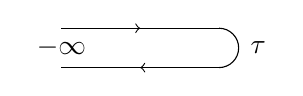
\begin{tikzpicture}
      \draw [->] (0,0) -- (1,0);
      \draw (0,0) -- (2,0);
      \draw (0,-0.5) -- (2,-0.5);
      \draw [->] (2,-0.5) -- (1,-0.5);
      \draw (2,-0.5) arc (-90:90:0.25) node at (2.5,-0.25) {$\tau$};
      \node at (0,-0.25) {$-\infty$};
  \end{tikzpicture}
  \caption{The time-loop integration path in the $S$ matrix.}
  \label{f2.11}
\end{marginfigure}

Considering the time-loop expansion for the $S$ Matrix
\begin{equation}
  \label{2.142}
  S(-\infty,-\infty) = T_s \exp [-i \int_{loop} d s_1 \hat{V}(s_1)]
\end{equation}
The integration path is the time loop in Fig.~\ref{f2.11}. The variable $s_1$ goes $(-\infty , \tau)$ and then $(\tau,-\infty)$. The operator $T_s $ orders along the entire loop, with earliest value of $s_1$ occurring first.
In expanding the $S$ matrix, Green's functions are encountered of the form
\begin{equation}
  \label{2.143}
  G(\lambda,s_1-s_2) = -i\bra{\phi_0}T_s C_\lambda(s_1) C_\lambda^\dagger(s_2) \ket{\phi_0}
\end{equation}
where $s_1$ and $s_2$ can be in different place of Fig.\ref{f2.11}.

\subsection{Six Green's Functions}
For the time-loop expansion, it is necessary to define six different Green's function even through they are not independent.
The six functions are
\begin{eqnarray}
  G^>(x_1,x_2) &=& -i\langle \psi(x_1) \psi^\dagger(x_2) \rangle \nonumber \\
  G^<(x_1,x_2) &=& i\langle \psi^\dagger(x_2) \psi(x_1) \rangle \nonumber \\
  G_t(x_1,x_2) &=& \Theta(t_1-t_2) G^>(x_1,x_2) + \Theta(t_2-t_1)G^<(x_1,x_2) \nonumber \\
  G_{\bar{t}}(x_1,x_2) &=& \Theta(t_2-t_1) G^>(x_1,x_2) +\Theta(t_1-t_2) G^<(x_1,x_2) \nonumber \\
  G_{ret}(x_1,x_2) &=& G_t - G^< = G^> - G_{\bar{t}}  \nonumber \\
  G_{adv}(x_1,x_2) &=& G_t -G^> = G^< -G_{\bar{t}} \label{2.144}
\end{eqnarray}
For homogeneous systems in equilibrium, Green's function depend only upon the difference of the arguments.
Then the important quantities are the Fourier transforms
\begin{equation}
  \label{2.145}
  G(\bk,E) = \int d\br e^{-i\bk \cdot \br} \int dt e^{-iEt} G(\br,t)
\end{equation}
where $G$ represents any of the six functions.

Often the Hamiltonian $H$ can be solved exactly in terms of eigenfunctions $\phi_\lambda(\br)$ and eigenvalues $\varepsilon_\lambda$.
Two example are the electron in a magnetic field or a free particle.
It is useful to have the expressions for the Green's function in terms of these eigenfunctions.
They are derived by expanding the field operators in terms of eigenfunctions and creation and destruction operators\footnote{where we have $x_1 = (\br_1,t)$}:
\begin{eqnarray}
  \phi(x_1) &=& \sum_\lambda C_\lambda \phi_\lambda (\br_1) e^{-i\varepsilon_\lambda t} \nonumber \\
  \phi^\dagger (x_1) &=& \sum_\lambda C^\dagger_\lambda \phi^*_\lambda(\br_1) e^{i\varepsilon_\lambda t} \label{2.146}
\end{eqnarray}
Then the Green's function in \eqref{2.144} are evaluated with the occupation faction $\eta_\lambda=\langle C^\dagger_\lambda C_\lambda \rangle$ and $t= t_1 -t_2$, we have
\begin{eqnarray}
  G^>(x_1,x_2) &=& -i \sum_\lambda (1-\eta_\lambda) \phi_\lambda(\br_1) \phi^*_\lambda(\br_2) e^{-i\varepsilon_\lambda t} \nonumber \\
  G^<(x_1,x_2) &=& i \sum_\lambda \eta_\lambda \phi_\lambda(\br_1) \phi^*_\lambda(br_2) e^{-i\varepsilon_\lambda t} \nonumber \\
  G_t(x_1,x_2) &=& -i \sum_\lambda [\Theta(t)-\eta_\lambda] \phi_\lambda(\br_1) \phi_\lambda^*(br_2) e^{-i\varepsilon_\lambda t} \nonumber \\
  G_{\bar{t}}(x_1,x_2) &=& -i \sum_\lambda [\Theta(-t)-\eta_\lambda] \phi_\lambda(\br_1) \phi_\lambda^*(br_2) e^{-i\varepsilon_\lambda t} \nonumber \\
  G_{ret} (x_1,x_2) &=& -i\Theta(t) \sum_\lambda \phi_\lambda(\br_1) \phi^*_\lambda(\br_2)e^{-i\varepsilon_\lambda t} \nonumber \\
  G_{adv} (x_1,x_2) &=& i\Theta(-t) \sum_\lambda \phi_\lambda(\br_1) \phi_\lambda^*(\br_2) e^{-i\varepsilon_\lambda t} \label{2.147}
\end{eqnarray}
at zero temperature $\eta_\lambda = \Theta(-\xi_\lambda)$ is the step function depending upon $\xi_\lambda = \varepsilon_\lambda - \mu$.
However these formulas are also valid in equilibrium at nonzero temperature.

The starting point for any calculation, is the behavior of the Green's functions for system without interaction.
Then the quantum number $\lambda$ becomes the wave vector $\bk$ and spin index $\sigma$.
The eigenvalue combination is $\phi_\lambda(\br_1)\phi^*_\lambda(\br_2) = \exp[i\bk \cdot (\br_1-\br_2)]/v$.
In noninteracting system in equilibrium, for \eqref{2.145}, with Fourier transformation give the free-particle Green's functions
\begin{eqnarray}
  G^>_0(\bk,t) &=& -i[1-\eta_\bk] e^{i\varepsilon_\bk t} \nonumber \\
  G^<_0(\bk,t) &=& i\eta_\bk e^{-i\varepsilon_\bk t} \nonumber \\
  G^0_t(\bk,t) &=& -i[\Theta(t) -\eta_\bk] e^{-i \varepsilon_\bk t} \nonumber \\
  G^0_{\bar{t}}(\bk,t) &=& -i [\Theta(-t)- \eta_\bk] e^{-i\varepsilon_\bk t} \nonumber \\
  G^0_{ret}(\bk,t) &=& -i \Theta(t) e^{-i\varepsilon_\bk t} \nonumber \\
  G^0_{adv}(\bk,t) &=& i\Theta(-t) e^{-i\varepsilon_\bk t} \label{2.148}
\end{eqnarray}
with Fourier transformation and $i\delta$ infinitesimal quantity
\begin{eqnarray}
  G^>_0(\bk,E) &=& -2\pi i [1-\eta_\bk] \delta(E-\varepsilon_\bk) \nonumber \\
  G^<_0(\bk,E) &=& 2\pi i \eta_\bk \delta(E-\varepsilon_\bk) \nonumber \\
  G_{ret}^0 (\bk,E) &=& \frac{1}{E-\varepsilon_\bk + i \delta} \nonumber \\
  G_{adv}^0 (\bk,E) &=& \frac{1}{E- \varepsilon_\bk - i \delta} \nonumber \\
  G_t^0 (\bk,E) &=& G_{ret}^0 + G^<_0 = \frac{1}{E-\varepsilon_\bk + i \delta_\bk} \nonumber \\
  G_{\bar{t}}^0 (\bk,E) &=& G^<_0 - G_{adv}^0 = \frac{-1}{E- \varepsilon_\bk - i\delta_\bk}  \label{2.149}
\end{eqnarray}
The time-order function $G^0_t$ is exactly the same on in \eqref{2.65}.
Note the two kinds of infinitesimal delta, where $\delta_\bk\equiv \delta \mathrm{sign}(\bk-\bk_F)$.

The above Green's functions are suitable for particles such as electrons or holes in semiconductors.
Another type of Green's function is needed for boson fields such as photons and phonons.
For phonons let $Q(x)$ be the displacement from equilibrium of the ions in the solid at position $x=(\br,t)$ in spacetime.
The phonon Green's functions are defined as
\begin{eqnarray}
  D^>(x_1,x_2) &=& -i \langle Q(x_1) Q(x_2) \rangle \nonumber \\
  D^<(x_1,x_2) &=& -i \langle Q(x_2) Q(x_1) \rangle \nonumber \\
  D_t(x_1,x_2) &=& \Theta(t_1-t_2) D^>(x_1,x_2) + \Theta(t_2-t_1) D^<(x_1,x_2) \nonumber \\
  D_{\bar{t}} (x_1,x_2) &=& \Theta(t_2-t_1) D^>(x_1,x_2) + \Theta(t_1-t_2) D^<(x_1,x_2) \nonumber \\
  D_{ret} &=& D_t-D^< = \Theta(t_1-t_2) [D^>-D^<] \nonumber \\
  D_{adv} &=& D_t-D^> = -\Theta(t_2-t_1) [D^> -D^<] \label{2.150}
\end{eqnarray}
There expressions are rather similar to those in \eqref{2.144} for particles.
The main difference is that $D^<$ and $D^>$ have the same sign, since no changer is made when interchanging the positions of boson operators.
Also the \textit{displacement operator is Hermitian}, $Q^\dagger = Q$, which introduces some redundancy such as $D^<(x_1,x_2) = D^>(x_2,x_1)$.

The displacement operators $Q$ are usually represented in terms of phonon raising and lowing operators.
Usually, we have $A_\bq = a^\dagger_{-\bq} + a_\bq$  in the definition of the phonon Green's function.
In this representation, the phonon Green's functions in equilibrium are expressed in terms of the phonon occupation number $N_\bq = \langle a^\dagger_\bq a_\bq \rangle$.
The noninteracting results are
\begin{eqnarray}
D^>(\bq,t) &=& -i[(N_\bq+1)e^{-i\omega_\bq t}+ N_\bq e^{i\omega_\bq t}]\nonumber \\
D^<(\bq,t) &=& -i[(N_\bq+1)e^{i\omega_\bq t} + N_\bq e^{-i\omega_\bq t}] \nonumber \\
D_{ret}(\bq,t) &=& -2\Theta(t) \sin(\omega_\bq t) \nonumber\\
D_{adv}(\bq,t) &=& -2\Theta(-t) \sin(\omega_\bq t) \\
D_t(\bq,t) &=& -i\lbrace(N_\bq + \Theta(-t))e^{i\omega_\bq t} + [N_\bq + \Theta(t)] e^{-i\omega_\bq t}\rbrace \nonumber\\
D_{\bar{t}}(\bq,t) &=& -i\lbrace(N_\bq + \Theta(t))e^{i\omega_\bq t} + [N_\bq + \Theta(-t)] e^{-i\omega_\bq t}\rbrace 	\nonumber\label{1.150}
\end{eqnarray}

\subsection{Dyson's Equation}
Each of the six Green's functions can be evaluated for an interacting system in terms of the $S$ matrix in \eqref{2.142}.

The potential $V$ is composed of electron, phonon, or photon opertors.
The operators are paired using Wick's theorem.
Each pair will have a time argument such as $G(s_i,s_j)$.
If both $s_i$ and $s_j$ are in the top loop, the expression is just the time-ordered Green's function.
If they are both in the return loop, the expression is the anti-time-ordered Green's function.
If one $s$ is on the top and other is in the bottom, then $T_s$ operator makes the expression be either $G^<$ or else $G^>$.
These relationships are shown in Fig.~\ref{f2.12}.
The $n$th term in the Green's function expansion is a product of $(n+1)$ factors, where each factor is on the the four Green's functions in Fig.~\ref{f2.12}.

\begin{figure}
\centering
\begin{tikzpicture}
      \draw (0,0)--(1,0);
      \draw (1,-0.5) arc (-90:90:0.25);
      \draw [middlearrow=latex] (1,-0.5)--(0,-0.5);
      \node at (0.4,0) {$\times$};
      \node at (0.8,0) {$\times$};
      \node [right] at (1.2,-0.25) {$G_t$};

      \draw [middlearrow=latex] (0,-1)--(1,-1);
      \draw (1,-1.5) arc (-90:90:0.25);
      \draw  (1,-1.5)--(0,-1.5);
      \node at (0.4,-1.5) {$\times$};
      \node at (0.8,-1.5) {$\times$};
      \node [right] at (1.2,-1.25) {$G_{\bar{t}}$};

      \draw [middlearrow=latex] (2,0)--(3,0);
      \draw (3,-0.5) arc (-90:90:0.25);
      \draw (3,-0.5)--(2,-0.5);
      \node at (2.8,0) {$\times$};
      \node at (2.8,-0.5) {$\times$};
      \node [right] at (3.2,-0.25) {$G^<$};
      \node [above] at (2.8,0) {$s_1$};
      \node [below] at (2.8,-0.5) {$s_2$};

      \draw (2,-1)--(3,-1);
      \draw (3,-1.5) arc (-90:90:0.25);
      \draw [middlearrow=latex] (3,-1.5)--(2,-1.5);
      \node at (2.2,-1) {$\times$};
      \node at (2.8,-1.5) {$\times$};
      \node [right] at (3.2,-1.25) {$G^>$};
      \node [below] at (2.8,-1.5) {$s_1$};
      \node [above] at (2.2,-1) {$s_2$};
\end{tikzpicture}
  \caption{The four Green's function $G(s_1,s_2)$ depend on whether the time variable are on the outgoing or return parts of the time loop. }
  \label{f2.12}
\end{figure}

Considering an example. Below is given a potential term $V$ of the type found for \textit{electrons scattering from impurities}.
The first term in the $S$-matrix expansion for $G^<$ with this interaction is
\begin{eqnarray} \label{2.154}
V &=& \sum_{\alpha \beta} M_{\alpha\beta} C^\dagger_\alpha C_\beta \nonumber \\
G^<(\lambda,t_1-t_2) &=& G^<_0(\lambda,t_1-t_2) \\
&+& \sum_{\alpha\beta}M_{\alpha\beta} \int ds \bra{\phi_0} T C^\dagger_\lambda(t_2) C_\beta (s) \ket{\phi_0} \bra{\phi_0} TC^\dagger_\alpha(s) C_\lambda(t_1) \ket{\phi_0} \nonumber
\end{eqnarray}
The $s$ integral runs over the time loop.
For $G^<$ there are two possibilities, where $s$ is on the top or below of the loop.
\begin{equation}
  G^<(\lambda,t_1-t_2) = G_0^<(\lambda,t_1-t_2) + M_{\lambda\lambda} \int_{-\infty}^\infty ds [G^0_t(\lambda,t_1-s)G_0^<(\lambda,s-t_2)
  - G_0^<(\lambda,t_1-s)G^0_{\bar{t}}(s-t_2)] \label{2.155}
\end{equation}
A sign change occurred in the last term when the direction of the time integration was changed from $(\infty,-\infty)$ to $(-\infty,\infty)$.

In the expansion of the $S$ matrix, each time integral produces one set of terms for the outward $s$ leg, and another for the return leg.
The $n$th term in the $S$-matrix expansion produce $2^n$ arrangements.
All of there terms can be managed by using a matrix formulation
\begin{eqnarray} \label{2.156}
  G =
  \begin{bmatrix}
  G_t & -G^<\\
  G^> & -G_{\bar{t}}
  \end{bmatrix}
  ~ ~ ~ ~
  \Sigma =
  \begin{bmatrix}
  \Sigma_t & -\Sigma^< \\
  \Sigma^> & -\Sigma_{\bar{t}}
  \end{bmatrix}
\end{eqnarray}

For systems either in equilibrium or non-equilibrium, Dyson's equation is most easily expressed by using the matrix notation
\begin{eqnarray}
  G(x_1,x_2) &=& G_0(x_1-x_2) + \int_{-\infty}^\infty dx_3 \int_{-\infty}^\infty dx_4 G_0(x_1-x_3) \nonumber \\
  &\times& \Sigma(x_3,x_4) G(x_4,x_2) \label{2.157}
\end{eqnarray}
The matrix formulation comes directly from the time loop.
Each $s$ integral in the $S$ matrix has an outward and return leg.
Each of these legs gives a different Green's function. So each time integral generates two Green's function.

With a simple notation where the product of two functions implies an integration over the four variable $dx$, which condenses the Equation
\begin{equation}
  G = G_0 + G_0 \Sigma G \label{2.158}
\end{equation}
Then the equation are iterated.
The following exact expressions are:
\begin{eqnarray}
  G_{ret} &=& G_{ret}^0[1+\Sigma_{ret}G_{ret}] \nonumber \\
  G_{adv} &=& G_{adv}^0[1+\Sigma_{adv}G_{adv}] \nonumber \\
  G^> &=& [1+G_{ret}\Sigma_{ret}]G^>_0[1+\Sigma_{adv}G_{adv}] + G_{ret} \Sigma^>G_{adv} \nonumber \\
  G^< &=& [1+G_{ret}\Sigma_{ret}]G^<_0[1+\Sigma_{adv}G_{adv}] + G_{ret} \Sigma^<G_{adv} \nonumber \\
  G_t &=& [1+G_{ret}\Sigma_{ret}]G^0_t[1+\Sigma_{adv}G_{adv}] + G_{ret} \Sigma_{\bar{t}}G_{adv} \nonumber \\
  G_{\bar{t}} &=& [1+G_{ret}\Sigma_{ret}]G^0_{\bar{t}}[1+\Sigma_{adv}G_{adv}] + G_{ret} \Sigma_tG_{adv} \label{2.159}
\end{eqnarray}
With the Fourier transformation, and the spectral function, $A(\bk,\omega) = -2ImG_{ret}(\bk,\omega)$,
\begin{eqnarray}
G_{ret}(k,\omega)&=& \frac{1}{\omega -\varepsilon_k -\Sigma_{ret}}, ~ ~ ~ \sigma = \omega -\varepsilon_k -Re[\Sigma_{ret}] \nonumber\\
G_{adv}(k,\omega)&=& \frac{1}{\omega -\varepsilon_k -\Sigma_{adv}}, ~ ~ ~ \Sigma_{adv}= \Sigma_{ret}^* \nonumber\\
A(k,\omega) &=& -2Im[G_{ret}(k,\omega)] = \frac{2\Gamma}{\sigma^2 +\Gamma^2}, ~ ~ ~ \Gamma = - Im[\Sigma_{ret}]>0 \nonumber\\
\Sigma^< &=& 2i \eta_F(\omega) \Gamma(k,\omega), ~ ~ ~ G^< = i\eta_F(\omega)A(k,\omega) \nonumber\\
\Sigma^>&=& -2i(1-\eta_F)\Gamma, ~ ~ ~ G^>=-i(1-\eta_F)A   \label{2.160}
\end{eqnarray}
More will discussed in next chapter.

\section{Photon Green's Functions}\label{s2.10}
Considering the interaction of charges with themselves and with the photon field\ref{s1.5}.
The interaction Hamiltonian for spinless particles in the non-relativistic limit
\begin{equation}
  H=\sum_i \frac{1}{2m}[\bp_i - \frac{e}{c} \mathbf{A}(\br_i)]^2 + \frac{1}{2} \sum_{i\neq j}\frac{e_i e_j}{r_{ij}} + \sum_{\bk \lambda} \omega_{\bk \lambda} a^\dagger_{\bk \lambda} a_{\bk \lambda} \label{2.161}
\end{equation}
With the vector potential is given by expansion\begin{eqnarray}
  \frac{1}{c}A_\mu &=& \frac{1}{\sqrt{v}} \sum_{\bk\lambda}e^{i\bk\cdot \br}A_\mu (\bk,\lambda,t) \label{2.162} \\
  A_\mu(\bk,\lambda,t) &=& (\frac{2\pi}{\omega_\bk})^{\frac{1}{2}} \xi_\mu(\bk ,\lambda) (a_{\bk\lambda}e^{-i\omega_\bk t} +a_{-\bk \lambda}^\dagger e^{i\omega_\bk t}) \label{2.163}
\end{eqnarray}
where $\bk$ is the wave vector and $\lambda$ is the polarization and $\mu$ is $x$,$y$ and $z$ component.
The operator $a_{\bk\lambda}$ obey boson statistics.
And Each state with $\bk$ and $\lambda$  has its own harmonic oscillator statistics.
The vector potential represents the photon field.
Two charges may interact via their common photon field or more directly through the instantaneous Coulomb interaction.
\textbf{The division of the interaction between photons and Coulomb field is arbitrary---- both interactions come from the same basic process.}
The Hamiltonian \eqref{2.161} is written in the Coulomb gauge, $\nabla \cdot \mathbf{A}=0$.
Another choice of gauge will result in a different division between photon and Coulomb,
The basic force between the particles are the same regardless of how the gauge is selected.

In terms of Green's function, for electron-electron interaction,
\begin{equation}
  v_q = \frac{4\pi e^2}{q^2} \label{2.165}
\end{equation}
is in fact just the Green's function of the longitudinal potential.
It has no frequency dependence because it is instantaneous.

Since $v_q$ is a Green's function, it has a Dyson equation
\begin{equation}
  v_q(\omega)= \frac{v_q}{1-v_q P(\bq,\omega)}  \label{2.167}
\end{equation}
The factor $P(\bq,\omega)$ is the \textbf{self-energy or polarization operator}.
Consider the Maxwell's equations in a homogeneous material with an isotropic dielectric constant $\epsilon$
\begin{eqnarray}
  \nabla \cdot \mathbf{B} &=& 0 \nonumber \\
  \nabla \times \mathbf{E} &=& 0 \nonumber \\
  \nabla \cdot \mathbf{E} &=& \frac{4\pi \rho}{\epsilon} \nonumber \\
  \nabla \times \mathbf{B} &=& \frac{\epsilon}{c} \partial_t \mathbf{E} + \frac{4\pi}{c} \mathbf{j} \label{2.168}
\end{eqnarray}
\marginnote{
Not quite understand here.
Since, usually $\nabla \times \mathbf{E} = -\frac{1}{c} \partial_t \mathbf{B}$.
For vacuum electromagnetic wave
\begin{eqnarray*}
  \nabla \cdot \mathbf{E} &=& 0 \\
  \nabla \cdot \mathbf{B} &=& 0 \\
  \nabla \times \mathbf{E} &=& -\partial_t \mathbf{B} \\
  \nabla \times \mathbf{B} &=& \mu_0 \epsilon_0 \partial_t \mathbf{E}
\end{eqnarray*}
}
For the scalar and vector potentials
\begin{eqnarray}
  \psi(\br) &=& \frac{1}{\epsilon} \int \frac{d^3 \br' \rho(\br')}{\abs{\br-\br'}} \nonumber \\
  \nabla^2\mathbf{A} - \frac{\epsilon}{c^2} \frac{\partial^2}{\partial t^2} \mathbf{A} &=& -\frac{4\pi}{c} \mathbf{j}_t  \label{2.169}
\end{eqnarray}
Here the Coulomb Green's function is
\begin{equation}
  \bar{v}_q = \frac{v_q}{\epsilon}  \label{2.170}
\end{equation}
Regarding \eqref{2.167}, it gives a formula for the dielectric function
\begin{equation}
  \epsilon(\bq,\omega) = 1 - v_q \mathbf{P}(\bq,\omega)  \label{2.171}
\end{equation}
This equation will serve as the definition of the longitudinal dielectric function.
It arises from the self-energy parts of the Coulomb potential.
The Green's function for the vector potential is
\begin{equation}
  D_{\mu\nu}(\bk,t-t') = -i\sum_\lambda \langle T A_\mu(\bk,\lambda,t) A_\nu(-\bk,\lambda,t')\rangle  \label{2.172}
\end{equation}
where $\mu$, $\nu$ are the $x,y,z$ components, with vector potential in \eqref{2.163}; the sum $\lambda$ is the sum over the two transverse polarizations of the light, while $\xi_\mu$ are the polarization vectors for each component.
At zero temperature,
\begin{equation}
  D^0_{\mu\nu}(\bk,t-t') = -\frac{2\pi i}{\omega_\bk} e^{i\omega_\bk \abs{t-t'}} \sum_\lambda \xi_\mu \xi_\nu \label{2.173}
\end{equation}
and with Fourier transform is
\begin{equation}\label{2.175}
  D^0(\bk,\omega) = \frac{4\pi}{\omega^2-\omega_\bk^2 + i\delta} \sum_\lambda \xi_\mu \xi_\nu = \frac{4\pi[\delta_{\mu\nu}-(k_\mu k_\nu/k^2)]}{\omega^2-\omega_\bk^2+ i\delta}
\end{equation}
This expression is referred to as the \textbf{photon Green's function}.
Keep in mind that the interaction between two charges occurs via both the scalar and vector potentials.
How the interaction is divided between scalar and vector potentials is somewhat arbitrary and is determined by the gauge condition.
After making this choice, the word "photon" is assigned to the vector potential part.
This division between photon and Coulomb is arbitrary, and both parts should really be viewed as arising from photons.

The photon Green's function also obeys a Dyson equation.
\begin{equation}
  D_{\mu\nu} = D^0_{\mu\nu} + \sum_{\lambda \delta} D^0_{\mu\lambda} \pi_{\lambda \delta} D_{\delta\nu}   \label{2.180}
\end{equation}
where $\pi_{\lambda \delta}(\bk,\omega)$ is the self-energy function, which is $3\times 3$ matrix.
